% !TEX root = ../../main.tex
% !TeX spellcheck = de_DE

\chapter{Ergebnisse}
Es werden 5 verschiedene Architekturen untersucht.
Dabei wird bei jeder Architektur die Modelle nach einem oder mehreren Merkmalen designt.
Damit sollen verschiedene Philosophien und Techniken verglichen werden.
Gleichzeit ist es Ziel, den Einfluss verschiedener Hyperparameter zu evaluieren.

\section{Dense GAN}
\label{section:dense-gan}
Das Dense GAN ist an einem Tutorial für das MNIST Datenset inspiriert.\todo{quelle}
Diese Architektur zeichnet vor allem aus, das zur Verarbeitung ausschließlich Dense-Layer zum Einsatz kommen.
Damit repräsentiert es als einziges Modell das Dense-Layer, da alle anderen Architekturen hauptsächlich auf Convolutional-Layer setzten.
Somit lässt sich ein interessanter Vergleich der Ergebnisse ziehen.

\subsection{Architektur}
Die Architektur wurde zu großen Teilen übernommen.
Jedoch wurde im Tutorial nur ein GAN ohne Konditionalisierung beschrieben.
Folglich fehlt das Label als Eingabe, was in der dieser Architektur ergänzt wird.
\newline

\subsubsection{Discriminator}
Der Input des Discriminators entspricht den klassischen CGAN.
Wie in der Abbildung \ref{architecture:densegan-dis-input} zu erkennen ist, wird der Label-Input auf die gleiche Größe wie der Bild-Input gebracht.
Anschließend werden beide Eingaben mit einer Multiply Schicht vereint.

\begin{figure}[H]
	\centering
	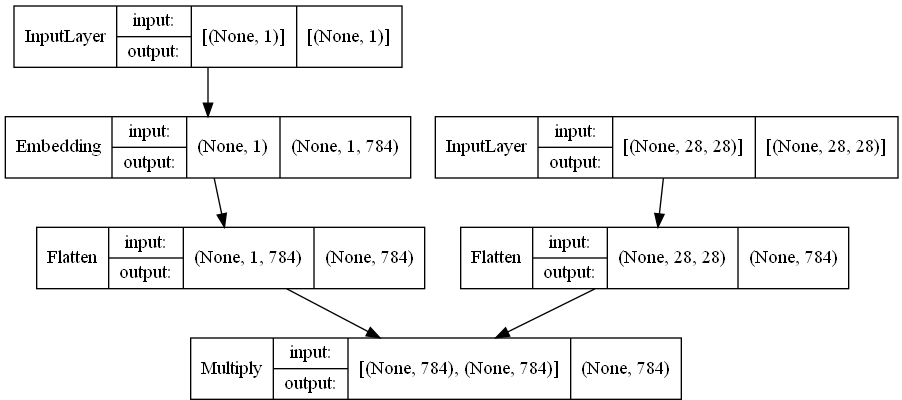
\includegraphics[height=0.3\textheight]{kapitel/5_ergebnisse/architectures/densegan_discriminator/inputs.png}
	\caption{Inputs des Dense-GAN-Discriminators}
	\label{architecture:densegan-dis-input}
\end{figure}

\subsubsection{Generator}

Sowohl die Architektur des Discriminators \cref{architecture:densegan-dis} als auch des Generators \cref{architecture:densegan-gen} ist in den Anlagen als volle Diagramme zu finden.

\subsection{Hyperparameter}
Für das Training wurde eine Anzahl an vordefinierten Hyperparameterkombinationen ausprobiert.

\begin{table}[H]
	\centering
	\begin{tabular}{l l}
		Name                        & Werte            \\ \hline
		Epochen                     & 100              \\
		Batch Size                  & 32, 64           \\
		Dropout                     & 0.2, 0.3, 0.4         \\
		Smoothness                  & 0, 0.1           \\
		Learning Rate Discriminator & 2e-3, 2e-4, 3e-4, 2e-5 \\
		Learning Rate Generator     & 2e-3, 2e-4, 3e-4, 2e-5
	\end{tabular}
	\caption{Hyperparameter für das Training des Dense-GANs}
\end{table}

\subsubsection{Ergebnisse}
\todo{long run}
\subsubsection{Zusammenfassung}


\section{DC-GAN-Late-Label}
\label{section:dc-gan-late-label}
Die Architektur dieses Modells basiert nicht auf anderen Papern oder Tutorials.
Stattdessen wird die Idee ausprobiert, die Convolutional Layer des Discriminators ausschließlich auf die Bilder anzuwenden.
Das Label wird dann erst im letzten Schritt mit dem Ergebnis der Convolutional Layer verknüpft und bewertet.
Die Entscheidung ist mit dem Verhalten der Convolutional Layern zu begründen.
Denn die Layer extrahieren Zusammenhänge von nebeneinanderliegenden Pixeln.
Diese Zusammenhänge sind jedoch nicht natürlich bei einem synthetischen Latent-Vektor gegeben.

\subsubsection{Architektur}
Die Besonderheit der Architektur liegt in der späten Fusionierung von Bild- und Labeldaten beim Discriminator.
Ein Diagramm mit der genauen Architektur befindet sich im Anhang (Discriminator \cref{architecture:dcgan-dis} und Generator \cref{architecture:dcgan-gen}).


Allgemein werden primär Convolutional und Convolutional Transposed Layer genutzt.
Beim Discriminator besteht eine Schicht aus einer Kombination von Conv2d, LeakyReLu (mit einem alpha von 0.2) und Dropout (beeinflusst vom Hyperparameter).
Der Generator besteht aus Schichten von Conv2DTranspose, BatchNormalisation und LeakyReLu (mit einem alpha von 0.2).

\subsubsection{Hyperparameter}
Die Hyperparameter werden mithilfe des Gridsearchverfahrens optimiert.
\begin{table}[H]
	\centering
	\begin{tabular}{l l}
		Name                        & Werte            \\ \hline
		Epochen                     & 100              \\
		Batch Size                  & 32, 64            \\
		Dropout                     & 0.3, 0.4         \\
		Smoothness                  & 0, 0.1           \\
		Learning Rate Discriminator & 2e-3, 2e-4, 3e-4 \\
		Learning Rate Generator     & 2e-3, 2e-4, 3e-4
	\end{tabular}
	\caption{Hyperparameter für das Training des 'DC-GAN-Late-Label's}
\end{table}

\subsubsection{Ergebnisse}
\begin{itemize}
	\item Tensorboard Graph -> beste Hyperparameter?
	\item 'beste' Bilder
\end{itemize}

\subsubsection{Zusammenfassung}
\todo{auf Hyperparameter eingehen + zu negativ?}
Wie anhand der Ergebnisse zu erkennen ist, sind die Trainingsergebnisse nicht mit den Originalbildern vergleichbar.
Es bestehen insbesondere keine Sensitivität gegenüber Labeln.
So wird keine Figur erkennbar abgebildet.
Stattdessen wird in der Regel eine Kombination aus Kreis und Quadrat in verschiedenen Größen und Positionen erzeugt.
\newline

Allerdings unterscheiden sich die Bilder voneinander.
Es existiert somit kein Mode-Collapse und folglich wird die Latent-Dim immer in Betracht gezogen.
Außerdem sind die Figuren ohne Rauschen gezeichnet.
Das bedeutet, es existieren keine einzelnen Pixel außerhalb oder innerhalb der Figur in der jeweils anderen Farbe.



\section{DC Generator und Dense Discriminator}
Das GAN bedient sich des Generators aus dem DC-GAN \cref{section:dc-gan-late-label} und dem Discriminator des Dense-GANs \cref{section:dense-gan}.
Beide Architekturen wurden zuvor schon verwendet und folglich nicht weiter angepasst werden.

\subsubsection{Architektur}
Die Architekturen für den Discriminator \cref{architecture:dcgen-densedis-dis} und Generator \cref{architecture:dcgen-densedis-gen} befinden sich im Anhang.
Es handelt sich um die gleichen Architekturen, ohne zusätzliche Änderungen.

\subsubsection{Hyperparameter}
\begin{table}[H]
	\centering
	\begin{tabular}{l l}
		Name                        & Werte            \\ \hline
		Epochen                     & 100              \\
		Batch Size                  & 16, 32           \\
		Dropout                     & 0.3, 0.4         \\
		Smoothness                  & 0, 0.1           \\
		Learning Rate Discriminator & 2e-3, 2e-4, 3e-4 \\
		Learning Rate Generator     & 2e-3, 2e-4, 3e-4
	\end{tabular}
	\caption{Hyperparameter für das Training vom DC-Discriminator und Dense-Generator}
\end{table}
\subsubsection{Ergebnisse}
\subsubsection{Zusammenfassung}

\section{Dense Generator und DC Discriminator}
Dieses GAN ist eine Kombination aus dem Dense GAN \cref{section:dense-gan} und DC GAN \cref{section:dc-gan-late-label}.
Dabei ist dem Dense GAN der Generator entnommen und dem DC GAN der Discriminator.
Beide Architekturen sind bereits an das Datenset angepasst und müssen nicht weiter verändert werden.

\subsubsection{Architektur}
Die Architekturen für den Discriminator \cref{architecture:densegen-dcdis-dis} und Generator \cref{architecture:densegen-dcdis-gen} befinden sich im Anhang.
Es wurden keine Änderungen zu den bereits vorhanden Architekturen vorgenommen.

\subsubsection{Hyperparameter}
\begin{table}[H]
	\centering
	\begin{tabular}{l l}
		Name                        & Werte            \\ \hline
		Epochen                     & 100              \\
		Batch Size                  & 16, 32           \\
		Dropout                     & 0.3, 0.4         \\
		Smoothness                  & 0, 0.1           \\
		Learning Rate Discriminator & 2e-3, 2e-4, 3e-4 \\
		Learning Rate Generator     & 2e-3, 2e-4, 3e-4
	\end{tabular}
	\caption{Hyperparameter für das Training vom Dense-Generator und DC-Discriminator}
\end{table}
\subsubsection{Ergebnisse}
\subsubsection{Zusammenfassung}

\section{DC-GAN-Medical-Inspired}

Die Architektur dieses Modells orientiert sich an einem Paper zu COVID Fällen \cite{inspiration-dc-gan-med}.
Bei den verwendeten Daten im Paper handelt es sich um schwarz-weiß Scans von Lungen zur Identifizierung von COVID-19 Erkrankungen.
Die Bilder sind deutlich größer als die von uns verwendeten, weshalb die Architektur dementsprechend angepasst werden muss.

\subsubsection{Architektur}
Sowohl Discriminator als auch Generator wurden aufgrund der anderen Bildgröße (244x244 anstatt 28x28 Pixel) angepasst.
Dafür wurde aber nur die Art des Paddings für die einzelnen Layer angepasst.
Die Architektur besteht dabei hauptsächlich aus Convolutional (Transpose) Layern.
Die Anzahl der Layer, die jeweiligen Ausgabedimensionen und Filtergrößen bleibt unverändert.
Dadurch entsteht ein vergleichsweise großes Netz.
Die genauen Architekturen befinden sich im Anhang, sowohl für den Discriminator \cref{architecture:dcgan-med-dis} als auch für den Generator \cref{architecture:dcgan-med-gen}.

\subsubsection{Hyperparameter}
\begin{table}[H]
	\centering
	\begin{tabular}{l l}
		Name                        & Werte            \\ \hline
		Epochen                     & 100              \\
		Batch Size                  & 16, 32           \\
		Dropout                     & 0.3, 0.4         \\
		Smoothness                  & 0, 0.1           \\
		Learning Rate Discriminator & 2e-3, 2e-4, 3e-4 \\
		Learning Rate Generator     & 2e-3, 2e-4, 3e-4
	\end{tabular}
	\caption{Hyperparameter für das Training des DC-GANs}
\end{table}

\subsubsection{Ergebnisse}
\begin{itemize}
	\item Tensorboard grafik
	\item Beste Bilder
	\item Hyperparameter Analyse
\end{itemize}
